\chapter{Ontwerp van de oplossing en de benodigde onderdelen}
\label{Ontwerp_van_de_oplossing_en_de_benodigde_onderdelen}
%%%%%%%%%%%%%%%%%%%%%%%%%%%%%%%%%%%%%%%%%%%%%%%%%%%%%%%%%%%%%%%%%%%%%%%%

%%%%%%%%%%%%%%%%%%%%%%%%%%%%%%%%%%%%%%%%%%%%%%%%%%%%%%%%%%%%%%%%%%%%%%%%
\section{Hardware}
%%%%%%%%%%%%%%%%%%%%%%%%%%%%%%%%%%%%%%%%%%%%%%%%%%%%%%%%%%%%%%%%%%%%%%%%

Het mechanisch ontwerp van de printer was grotendeels al gedaan, echter zijn er
een aantal aanpassingen gedaan, die staan hier beschreven.

%%%%%%%%%%%%%%%%%%%%%%%%%%%%%%%%%%%%%%%%%%%%%%%%%%%%%%%%%%%%%%%%%%%%%%%%
\subsection{Ge-3D-printe oplossingen}
%%%%%%%%%%%%%%%%%%%%%%%%%%%%%%%%%%%%%%%%%%%%%%%%%%%%%%%%%%%%%%%%%%%%%%%%

Een aantal problemen zijn opgelost door kleine onderdelen te 3D-printen. hier zijn
daar een paar voorbeelden van.

%%%%%%%%%%%%%%%%%%%%%%%%%%%%%%%%%%%%%%%%%%%%%%%%%%%%%%%%%%%%%%%%%%%%%%%%
\subsubsection{Voetjes van de printer}
%%%%%%%%%%%%%%%%%%%%%%%%%%%%%%%%%%%%%%%%%%%%%%%%%%%%%%%%%%%%%%%%%%%%%%%%

De voetjes van de printer waren te kort, dus daar zijn langere voor
ontworpen en ge-3D-print. Zie Figuur ~\ref{fig:voetjes} voor een render van
het \ac{3d} ontwerp.

\begin{figure}[h]
    \centerline{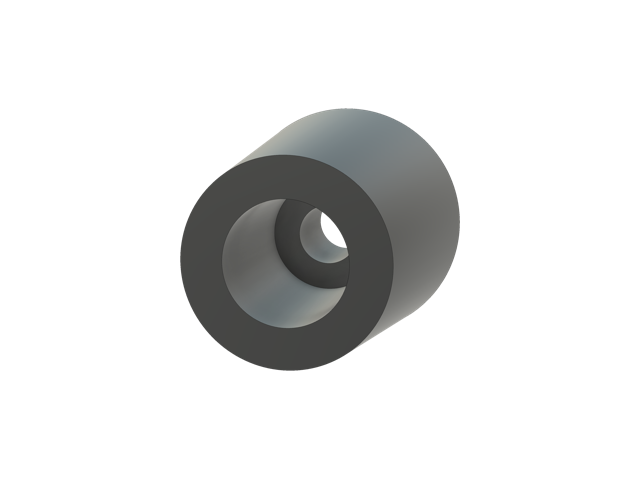
\includegraphics[width=0.45\textwidth]{voetjes}}
    \caption{Render van het \ac{3d} ontwerp van de voetjes van de printer}
    \label{fig:voetjes}
\end{figure}

%%%%%%%%%%%%%%%%%%%%%%%%%%%%%%%%%%%%%%%%%%%%%%%%%%%%%%%%%%%%%%%%%%%%%%%%
\subsubsection{Afstandhouder}
%%%%%%%%%%%%%%%%%%%%%%%%%%%%%%%%%%%%%%%%%%%%%%%%%%%%%%%%%%%%%%%%%%%%%%%%

De originele printer is omgebouwd met roestvrijstalen panelen aan alle kanten.
Om ervoor te zorgen dat er goede thermische isolatie is van de printkamer, is
het een dubbelwandig ontwerp met glaswol er tussen. De dubbele wanden worden op
afstand gehouden met ge-3D-printe afstandhouders. Zie Figuur
~\ref{fig:afstandhouder} voor een render van het \ac{3d} ontwerp van deze
afstandhouders.

%%%%%%%%%%%%%%%%%%%%%%%%%%%%%%%%%%%%%%%%%%%%%%%%%%%%%%%%%%%%%%%%%%%%%%%%
\subsubsection{Haakje}
%%%%%%%%%%%%%%%%%%%%%%%%%%%%%%%%%%%%%%%%%%%%%%%%%%%%%%%%%%%%%%%%%%%%%%%%

Om de deur dicht te houden is er een haakje geprint. Zie Figuur
~\ref{fig:haakje} voor een render van het \ac{3d} ontwerp van het haakje.

\begin{figure}[h]
    \centering
    \begin{minipage}{0.45\textwidth}
        \centerline{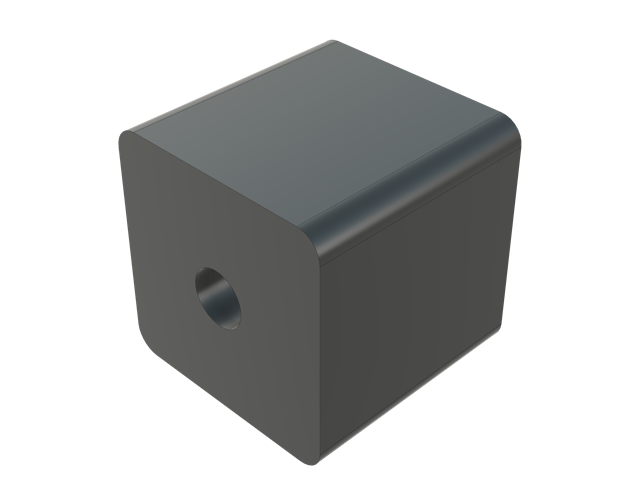
\includegraphics[width=0.9\textwidth]{afstandhouder}}
        \caption{Render van het \ac{3d} ontwerp van de afstandhouder van de printer}
        \label{fig:afstandhouder}
    \end{minipage}\hfill
    \begin{minipage}{0.45\textwidth}
        \centerline{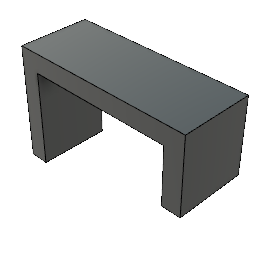
\includegraphics[width=0.9\textwidth]{haakje}}
        \caption{Render van het \ac{3d} ontwerp van het haakje van de printer}
        \label{fig:haakje}
    \end{minipage}
\end{figure}

%%%%%%%%%%%%%%%%%%%%%%%%%%%%%%%%%%%%%%%%%%%%%%%%%%%%%%%%%%%%%%%%%%%%%%%%
\subsubsection{DIN-rail bevestigingen}
%%%%%%%%%%%%%%%%%%%%%%%%%%%%%%%%%%%%%%%%%%%%%%%%%%%%%%%%%%%%%%%%%%%%%%%%

Op de zijkant van de printer was een DIN-rail bevestigd, hierop werd vervolgens
alle elektronica bevestigd. In Figuur ~\ref{fig:din1}, ~\ref{fig:din2} en
~\ref{fig:din3} zijn de montage stukken te zien voor de PCB en de
stroomtoevoer.

\begin{figure}[h]
    \centerline{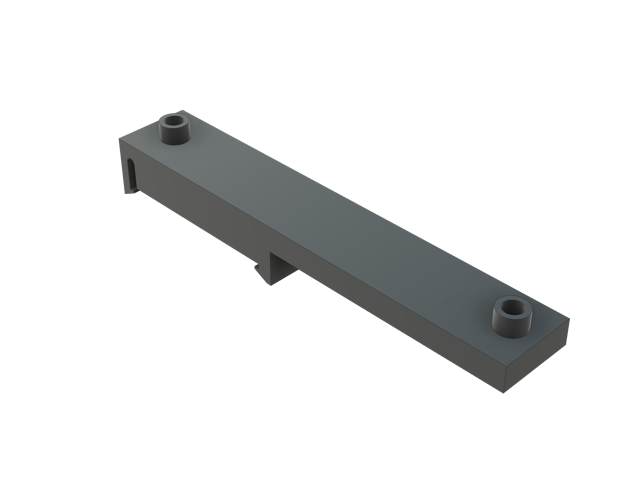
\includegraphics[width=0.45\textwidth]{pcb_mount}}
    \caption{Render van het \ac{3d} ontwerp van de DIN-rail PCB houder}
    \label{fig:din1}
\end{figure}

\begin{figure}[h]
    \centering
    \begin{minipage}{0.45\textwidth}
        \centerline{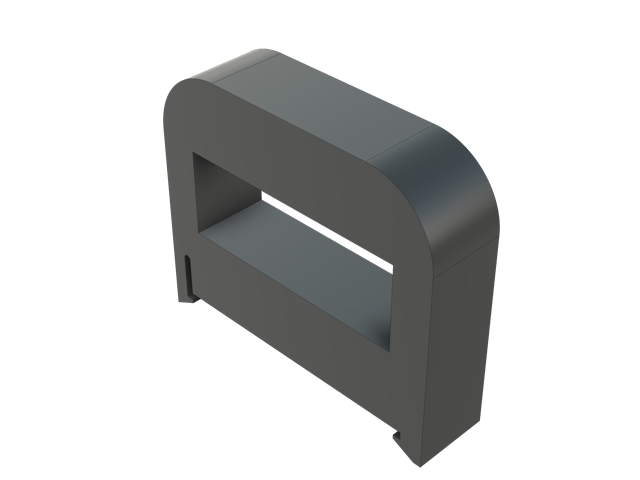
\includegraphics[width=0.9\textwidth]{io_switch_mount}}
        \caption{Render van het \ac{3d} ontwerp van de schakelaar houder op de DIN-rail}
        \label{fig:din2}
    \end{minipage}\hfill
    \begin{minipage}{0.45\textwidth}
        \centerline{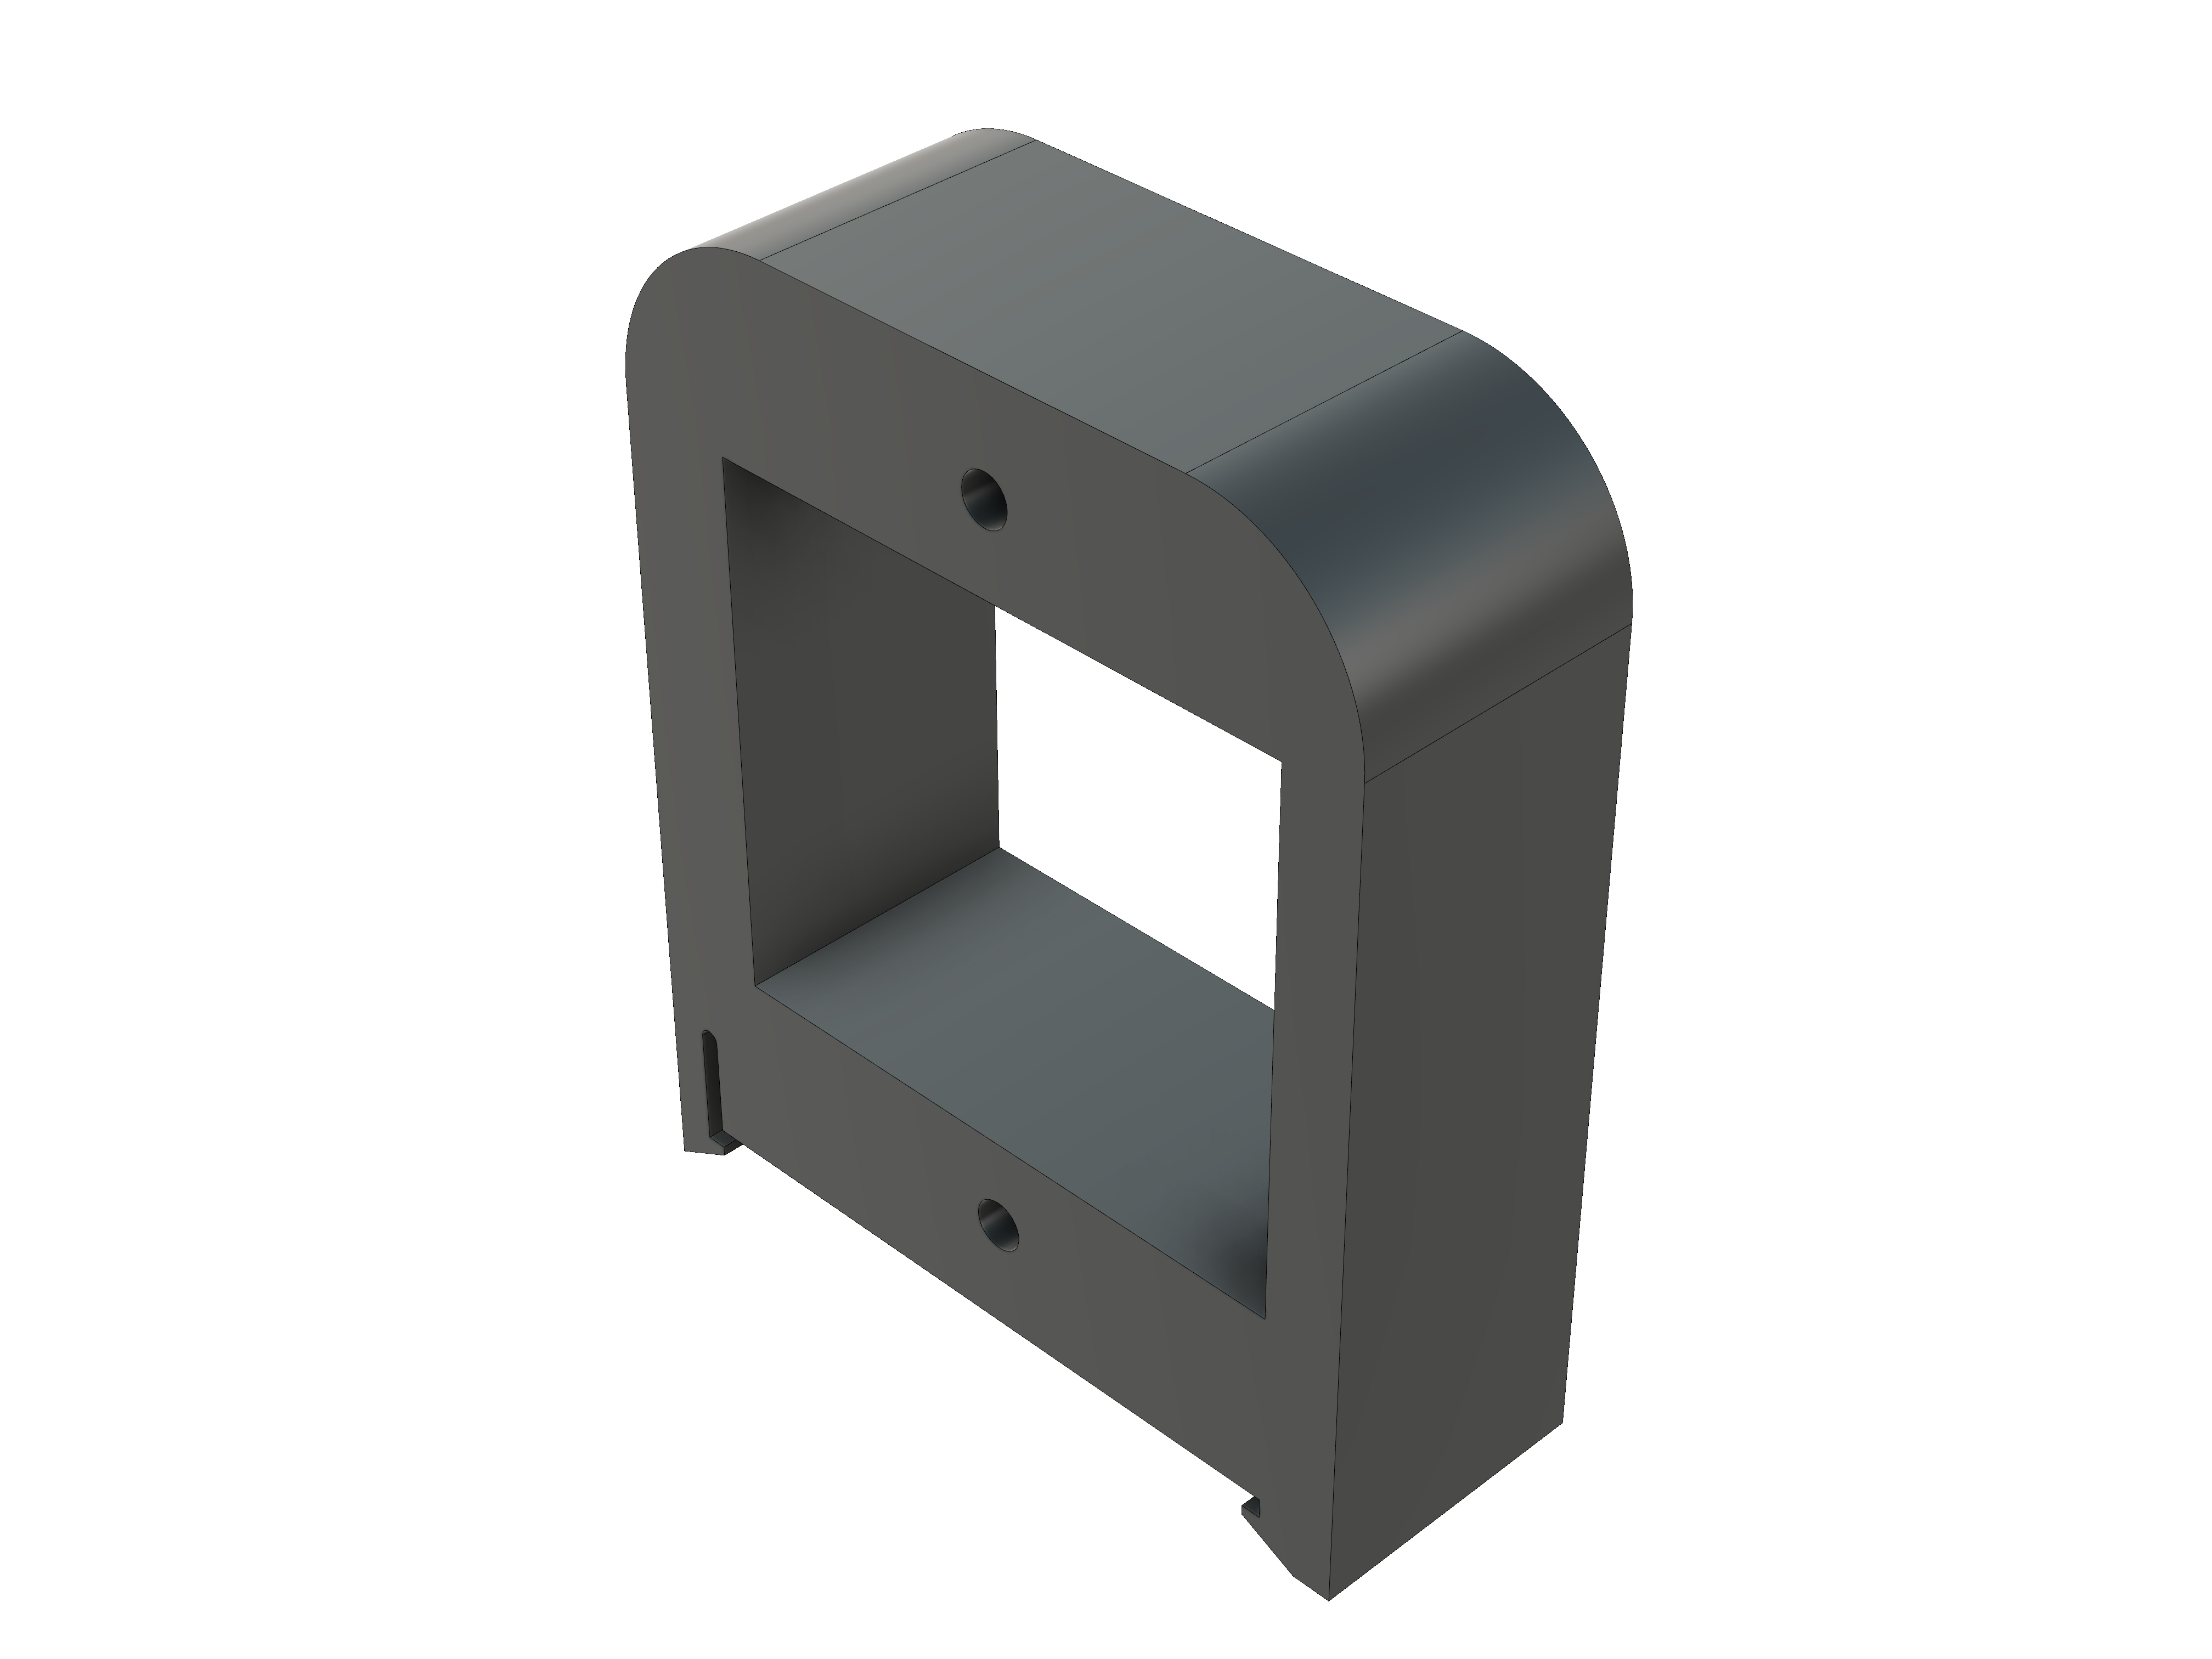
\includegraphics[width=0.9\textwidth]{c14_dinrail}}
        \caption{Render van het \ac{3d} ontwerp van het haakje van de C-14 houder op de DIN-rail}
        \label{fig:din3}
    \end{minipage}
\end{figure}


%%%%%%%%%%%%%%%%%%%%%%%%%%%%%%%%%%%%%%%%%%%%%%%%%%%%%%%%%%%%%%%%%%%%%%%%
\section{Electronica}
%%%%%%%%%%%%%%%%%%%%%%%%%%%%%%%%%%%%%%%%%%%%%%%%%%%%%%%%%%%%%%%%%%%%%%%%

De te gebruiken elektronica was grotendeels al vastgesteld voor het project
begon. Maar er was vrije keuze voor het hoofdboard, hiervoor is een
bigtreetech SKR-2 gekozen \cite{btt}. Dit board was gekozen omdat deze vrij
nieuw is, makkelijk te gebruiken, en veel mogelijkheden biedt.

%%%%%%%%%%%%%%%%%%%%%%%%%%%%%%%%%%%%%%%%%%%%%%%%%%%%%%%%%%%%%%%%%%%%%%%%
\section{Software}
%%%%%%%%%%%%%%%%%%%%%%%%%%%%%%%%%%%%%%%%%%%%%%%%%%%%%%%%%%%%%%%%%%%%%%%%]

Onder software word de slicer gezien. Er is gekozen voor prusaslicer, omdat dit
een veel gebruikte slicer is die veel opties biedt en gratis (open source) is.

De settings waarmee is getest zijn beschikbaar gesteld voor het team bij 3devo.
Zodat zij verder kunnen werken aan de progressie die tijdens de stageperiode is
verricht. Dit staat gedocumenteerd in de GitHub repo van het project.

%%%%%%%%%%%%%%%%%%%%%%%%%%%%%%%%%%%%%%%%%%%%%%%%%%%%%%%%%%%%%%%%%%%%%%%%
\section{Firmware}
%%%%%%%%%%%%%%%%%%%%%%%%%%%%%%%%%%%%%%%%%%%%%%%%%%%%%%%%%%%%%%%%%%%%%%%%

Voor de firmware is Marlin gekozen, en deze is geconfigureerd om te werken met
de hardware (elektronica/stappenmotoren/sensoren) van de printer. Dit staat
gedocumenteerd in de GitHub repo van het project.

%%%%%%%%%%%%%%%%%%%%%%%%%%%%%%%%%%%%%%%%%%%%%%%%%%%%%%%%%%%%%%%%%%%%%%%%
% \subsection{Subsection}
%%%%%%%%%%%%%%%%%%%%%%%%%%%%%%%%%%%%%%%%%%%%%%%%%%%%%%%%%%%%%%%%%%%%%%%%

